\section{Results}
\subsection{Impact of Directory Tree Structure}

The time taken to find the file in an uncached vs a cached filesystem image is shown in table \ref{Tab:tab1}. This constitues a speedup of 22.7X which is similar to what is reported in Figure 1 of the impressions paper. 

\begin{table}[ht]
    \caption{Results of Caching on the time to find a file}
    \begin{tabular}{|l|l|l|}
    \hline
     & Uncached & Cached \\ \hline
    Real Time to find file \\at depth 6 & 0m0.638s & 0m0.028s \\ \hline
    \end{tabular}
    \label{Tab:tab1}
    \end{table}

\subsection{Accuracy of Impressions in recreating file system properties}

The graphs from the experiments as mentioned in Figure two are shown in Figures:\ref{fig:a}, \ref{fig:b},\ref{fig:f}

\begin{figure}[htb]
	\center{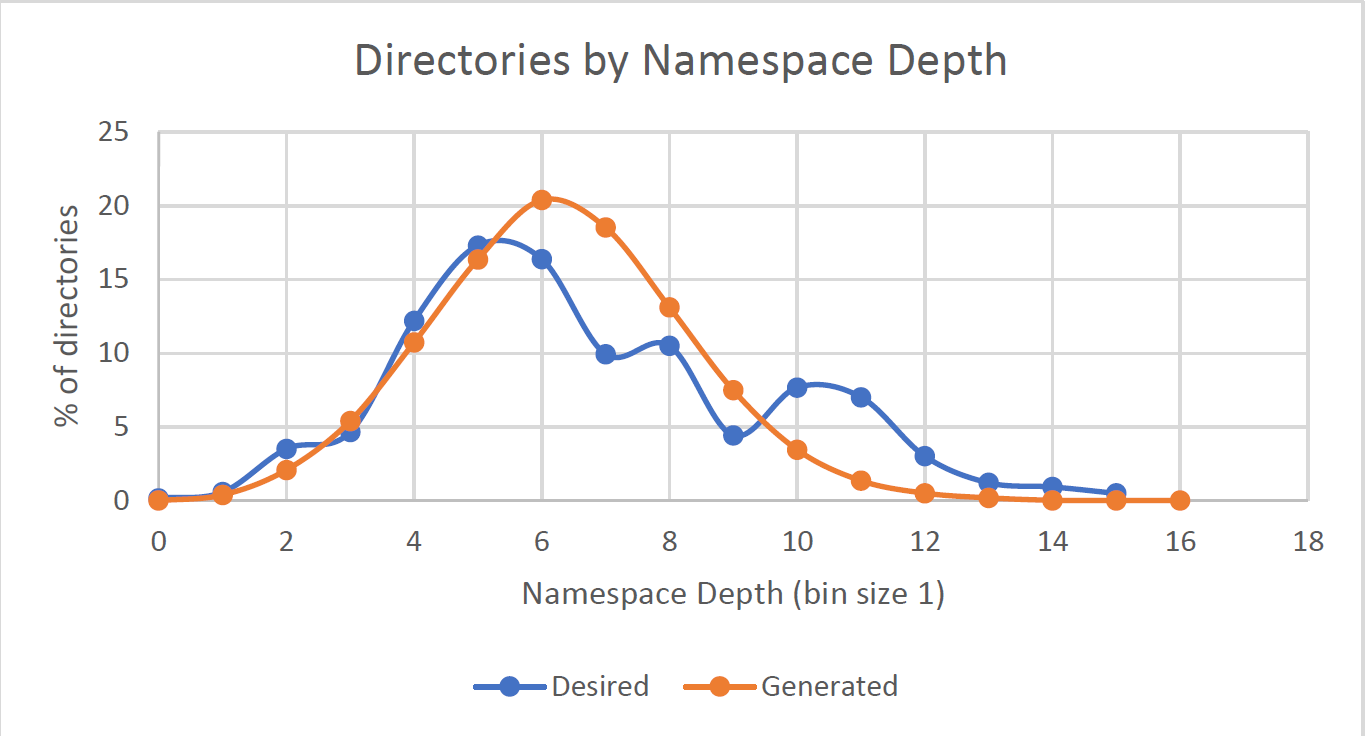
\includegraphics[width=0.5\textwidth]{a.PNG}}
	  \caption{\label{fig:a} Directories by Namespace Depth}
    \end{figure}

\begin{figure}[htb]
        \center{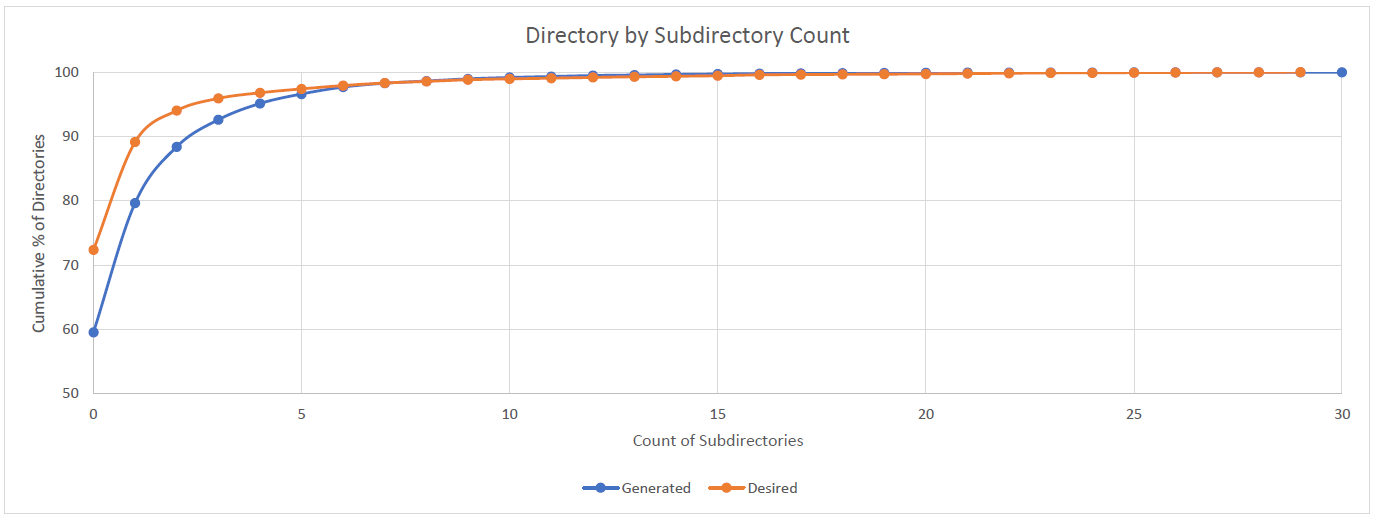
\includegraphics[width=0.5\textwidth]{b.PNG}}
          \caption{\label{fig:b} Directories by Subdirectory Count}
        \end{figure}

\begin{figure}[htb]
            \center{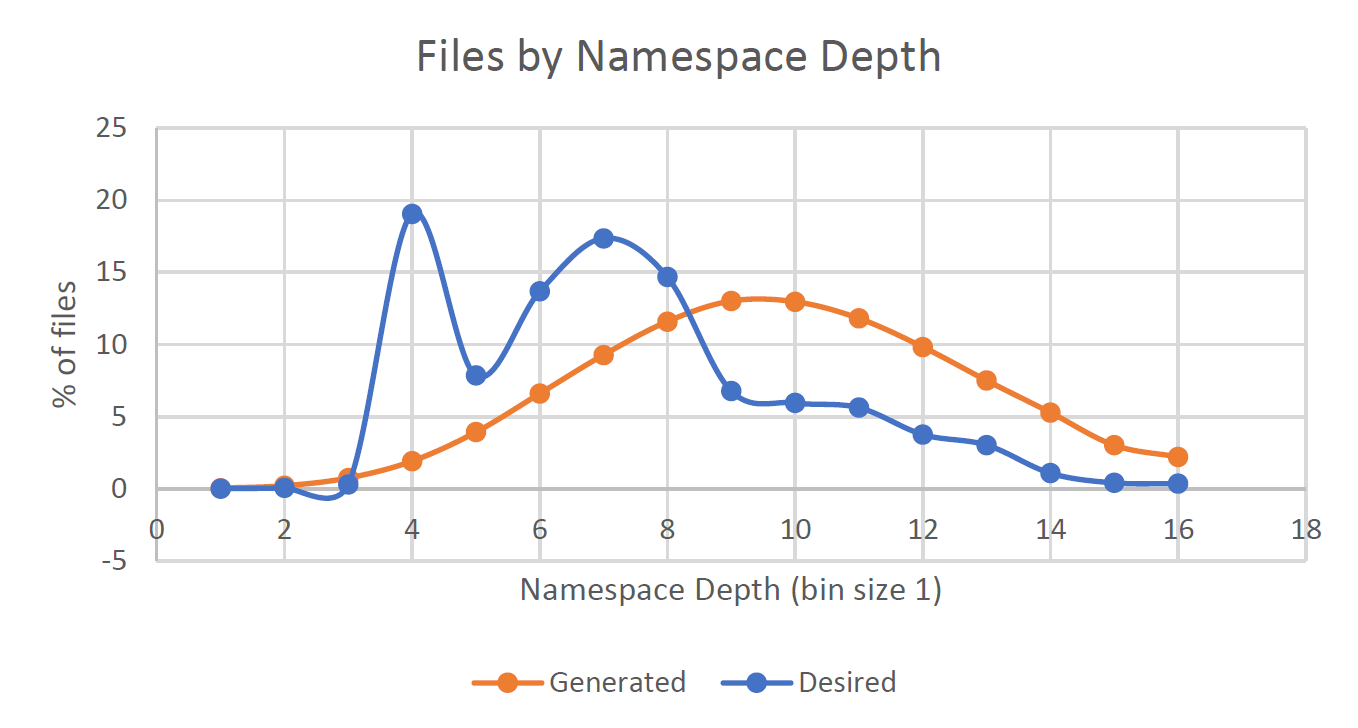
\includegraphics[width=0.5\textwidth]{f.PNG}}
              \caption{\label{fig:f} Files by Namespace Depth}
            \end{figure}

These results are not quite as close to the impressions results as I had expected them to be. I have a strong intuition that this is because I am comparing these results to a linux filesystem, and am including the \emph{many} executable files I have littered around in my home directory - I have many kernel source trees in the filesystem and that might explain some of the wierdness.